For the simulation of the Tritium-IFIC-2 prototype, $800$ fibers of $1~\mm$ diameter were arranged and uniformly distributed in sixteen different circles of increasing radius, as illustrated in Figure \ref{fig:FibersTritiumIFIC2Simulation}. The optical properties were included.

\begin{figure}[h]
\centering
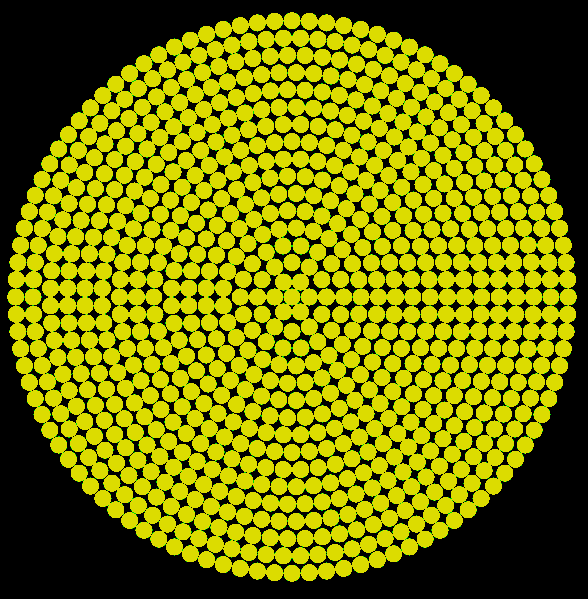
\includegraphics[scale=0.4]{6Simulations/62TRITIUMMonitor/621TRITIUMIFIC2/FiberDistribution_Tritium_IFIC_2_simulation.png}
\caption{Distribution of the scintillating fibers in the simulations of the Tritium-IFIC-2 prototype.\label{fig:FibersTritiumIFIC2Simulation}}
\end{figure}
The tritiated water source consists of a tritiated water volume with a thickness of $5~\mu\meter$ around each scintillating fiber. Scintillating fibers are located in a PTFE vessel. Two PMMA windows of $5~\mm$ thickness located in both ends of the cylindrical vessel and an optical grease layer with a thickness of $0.5~\mm$ located on each PMMA windows were included. Two PMTs, model R8520-460 from Hamamatsu \cite{DataSheetPMTs}, were also simulated as photosensors. 

%The optical properties used for the tritiated water, PTFE vessel, PMMA windows and the optical grease, mentioned in section \ref{sec:Geant4Environment}, are included in this simulation. 

The geometry simulated for TRITIUM-IFIC-2 is shown in Figure \ref{fig:TritiumIFIC2Simulation} in which is shown the PMTs (black), the optical grease (blue), the PMMA windows (white), the tritiated water (green) and the scintillating fibers (yellow). In this image, the PTFE container is not drawn to allow its interior to be seen. Several volumes of tritiated water were also excluded to allow some scintillation fibers to be seen. The PMTs do not cover the entire active area formed by the scintillating fiber bundle. This fact produces that some phtons are not detected, slightly reducing the efficiency of the detector. In the future, possible solutions will be studied, such as the use of photosensors that covers that entire active.

\begin{figure}[h]
\centering
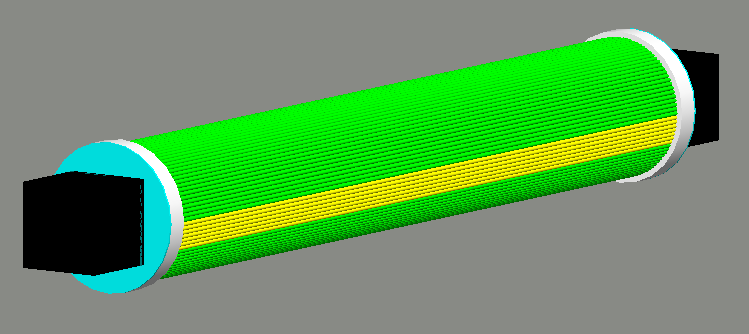
\includegraphics[scale=0.4]{6Simulations/62TRITIUMMonitor/621TRITIUMIFIC2/SimulationTritiumIFIC2.png}
\caption{Simulation of Tritium-IFIC-2 prototype. PMTs (black), the optical grease (blue), PMMA windows (white), tritiated water (green) and scintillating fibers (yellow). \label{fig:TritiumIFIC2Simulation}}
\end{figure}

The aim of these simulations were to find the activity resolution of the prototype and how it can be improved by increasing the integration time window and the number of prototypes read out in parallel. The detection of a tritium event in the TRITIUM-IFIC-2 prototype is shown in Figure \ref{fig:TritiumEventDetectedInSimulatedPrototype}. The paths of the photons created in scintillating fibers are represented by green lines ending in red dots when they are absorbed in the fiber or the water and blue dots when they are absorbed in the PMTs (detected). The fiber in which the tritium electron is detected is clearly identified. Some photons go out of the fiber and are not collected. Blue dots in both PMTs indicate that photons are detected in time coincidence.

\begin{figure}[hbtp]
\centering
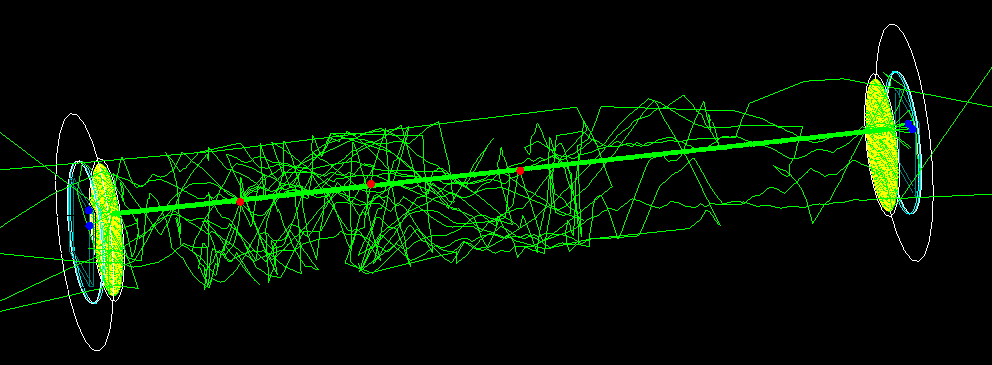
\includegraphics[scale=0.35]{6Simulations/62TRITIUMMonitor/621TRITIUMIFIC2/EventDetectedInTRITIUMIFIC2.png}
\caption{Tritium electron detected in the simulated TRITIUM-IFIC-2 prototype. The path of the optical photons is represented by green lines and the position in which they are absorbed is represented by red and blue dots (absorbed in water or PMT, respectively).\label{fig:TritiumEventDetectedInSimulatedPrototype}}
\end{figure}

Several variables were used to check the different steps of the simulation such as the production of tritium electrons, the energy deposition in scintillating fibers and their subsequent photon emission, the spatial distribution of generated events, the detected events, etc. The distribution of the number of photons detected by photosensors per tritium event for the TRITIUM-IFIC-2 prototype is shown in Figure \ref{fig:SimulatedPhotonsDetected}. A maximum of $17$ photons is obtained for the TRITIUM-IFIC-2 prototype simulations, which is in agreement with the distribution of photons per tritium event measured experimentally, shown in Figure \ref{fig:PhotonsPerTritiumEventIFIC2}. The experimental distributions are lower than the simulations mainly in the range from $3$ to $8$ photons per event, probably due to some subtle imperfections of the prototype, which are impossible to included in the simulations.

\begin{figure}[hbtp]
\centering
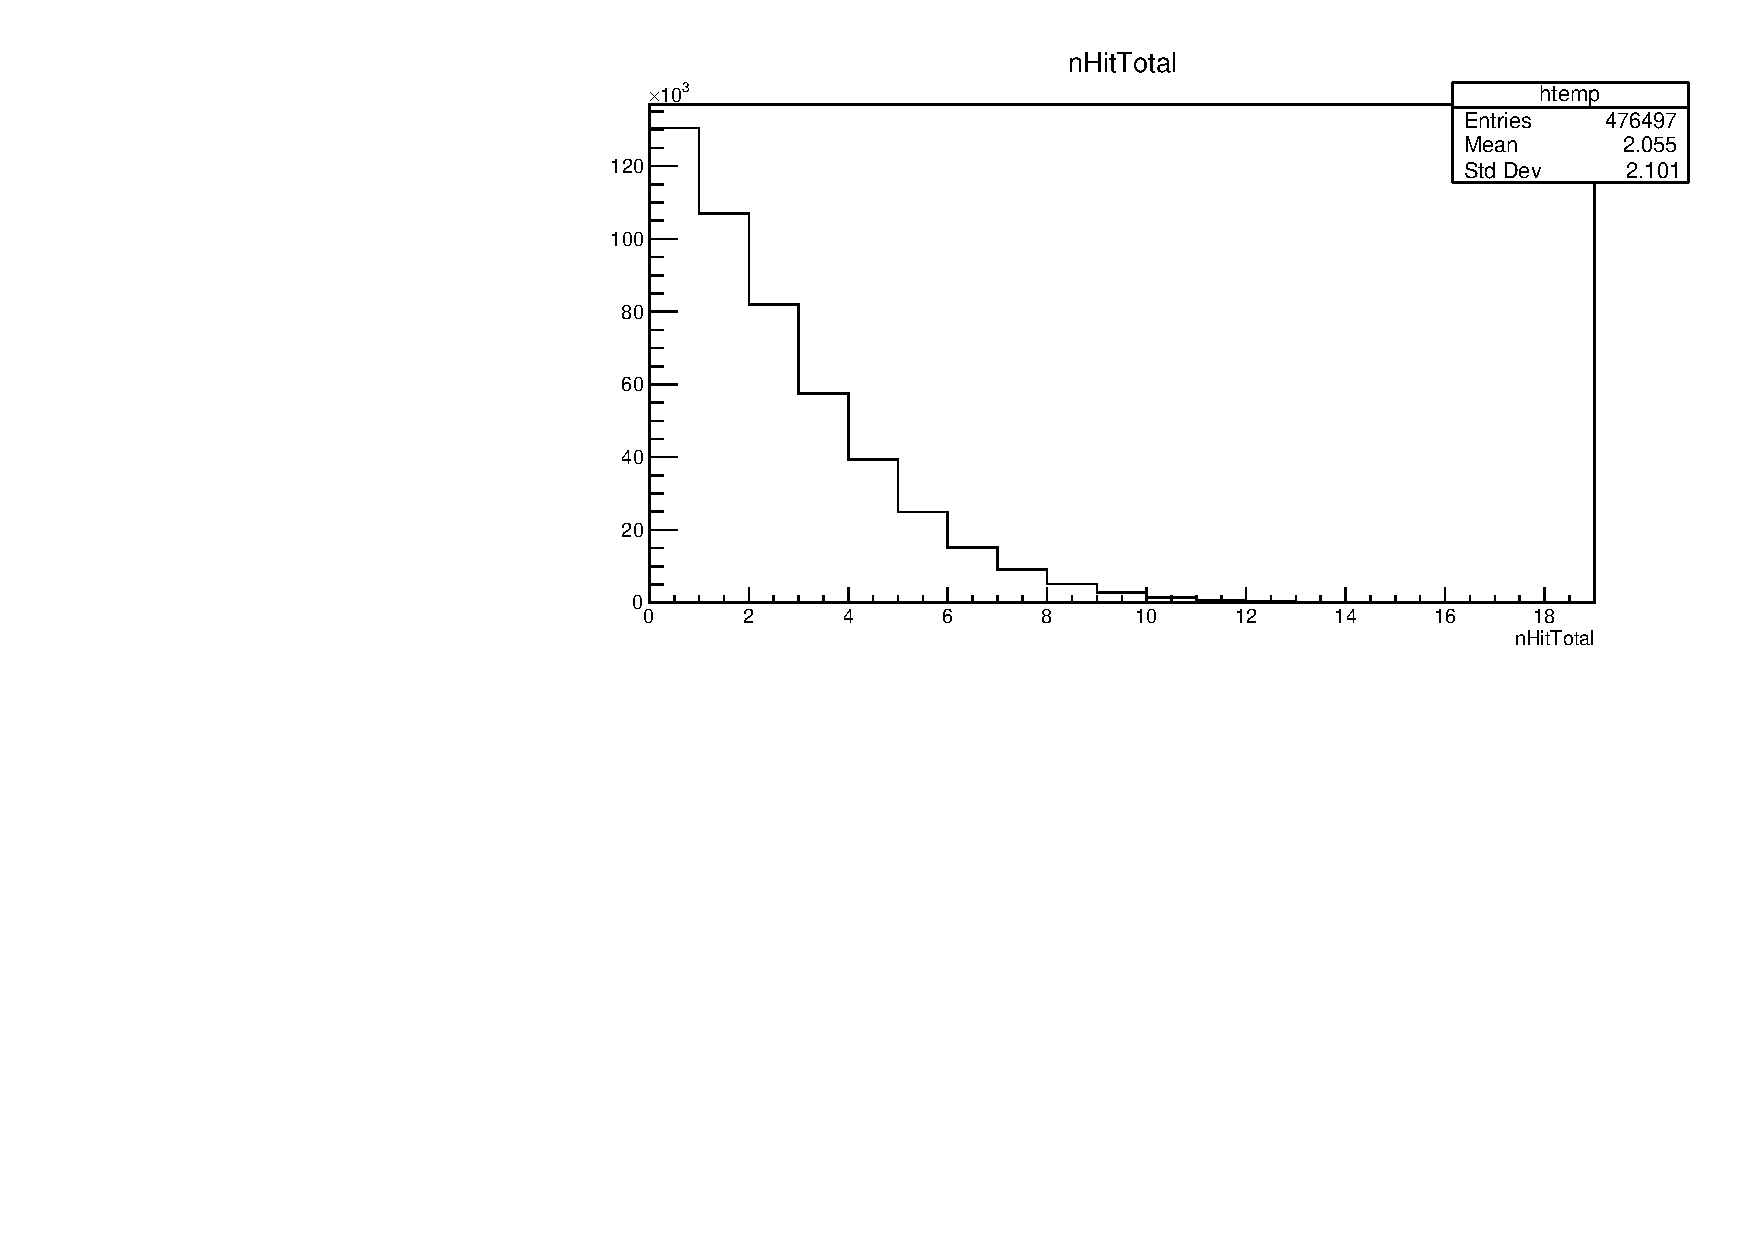
\includegraphics[scale=0.65]{6Simulations/62TRITIUMMonitor/621TRITIUMIFIC2/PhotonsDetected_simulation.pdf}
\caption{Photons detected by both PMTs per tritium event in the simulated TRITIUM-IFIC-2 prototype.\label{fig:SimulatedPhotonsDetected}}
\end{figure}

Activities from $100~\becquerel/\liter$ to $5~\kilo\becquerel/\liter$ for three months of data taking and an integration counting time of $10~\min$ were simulated. The simulation results are presented in Figure \ref{fig:1Det10Min250BqL}. A difference of $250~\becquerel/\liter$ in the activity is not distinguished due to the overlapping of distributions. To reduce the width of the distribution obtained for each activity, the statistics must be increased, which can be done in two different ways, either by increasing the integration time or the number of prototypes read out in parallel. To check the role of increasing the integration time, distributions for integration times of $10~\min$, $30~\min$ and $60~\min$ were generated. They are shown in Figure \ref{fig:1Det250BqLseveralTimes}. The effect of increasing the integration time is clearly visible in this figure, by reducing the relative distribution width and improving the activity resolution of the TRITIUM monitor. Differences as low as $250~\becquerel/\liter$ are clearly discriminated with only one TRITIUM-IFIC-2 module and an integration time of $60~\min$, which could still be considered as a quasi-real time measurement. Similarly, these distributions are shown in Figure \ref{fig:SeveralDet250BqL10min} for $10~\min$ of integration time, for 1, 5 and 10 modules read out in parallel. Again, the reduction of the distribution width with increasing number of modules is clearly visible in these figures, improving the activity resolution of the detector. In this case, differences of $250~\becquerel/\liter$ are clearly discerned by an integration time of $10~\min$ and 5 TRITIUM-IFIC-2 modules. The resolution, defined as
\begin{equation}
\text{Resolution(\%)}=\frac{\text{FWHM}}{\text{centroid}}\cdot{}100
\label{eq:Resolution}
\end{equation}
is plotted in Figure \ref{fig:Resolution}. It can be observed that the resolution improves with the integration time and the number of modules. Therefore, both parameters must be set according to the requirements and funding of the experiment. The studied cases are summarized in Table \ref{tab:DifferentCasesOfTI2}.


\begin{figure}
\centering
    \begin{subfigure}[b]{0.7\textwidth}
    \centering
    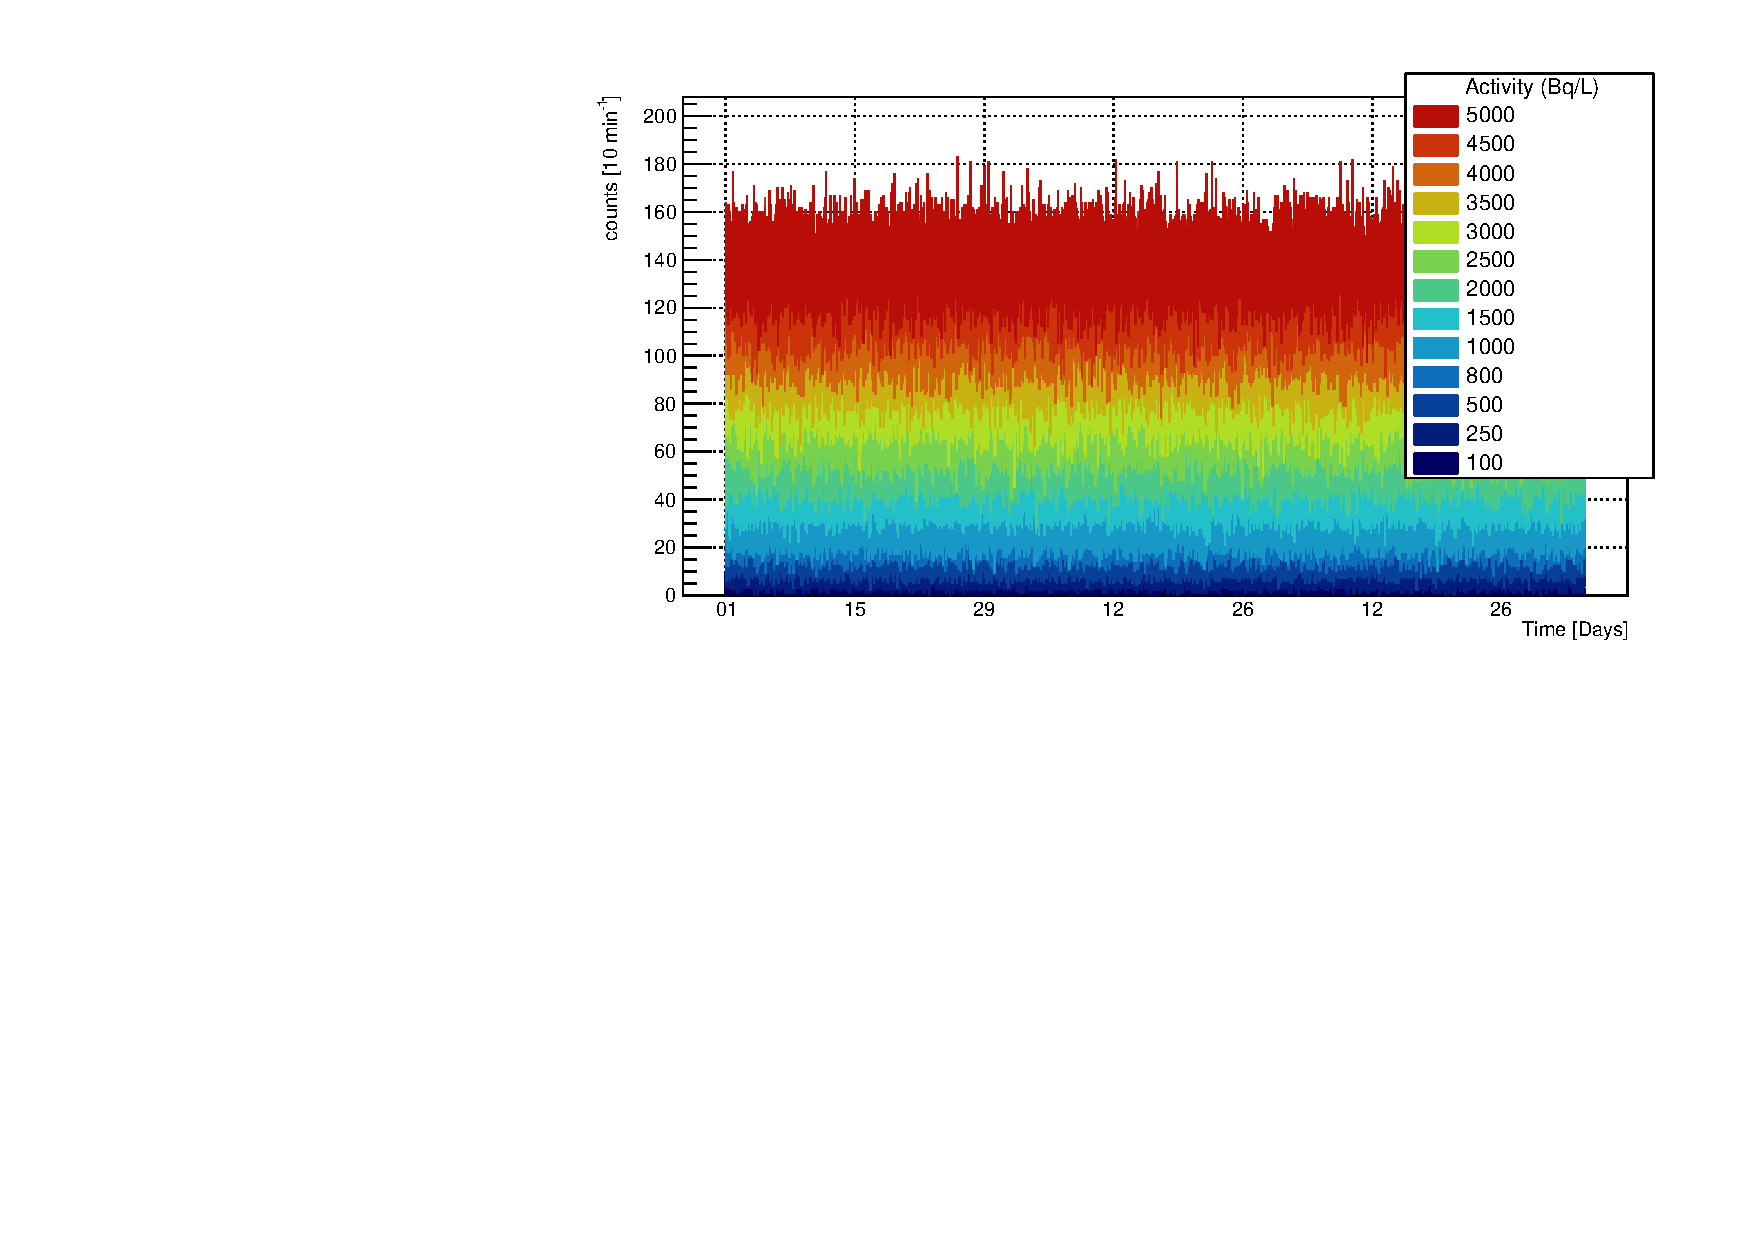
\includegraphics[width=\textwidth]{6Simulations/62TRITIUMMonitor/621TRITIUMIFIC2/RawData_1Det_10min_250BqL.pdf}  
    \caption{\label{subfig:RawData1Det10Min250BqL}}
    \end{subfigure}
    \hfill
    \begin{subfigure}[b]{0.7\textwidth}
    \centering
    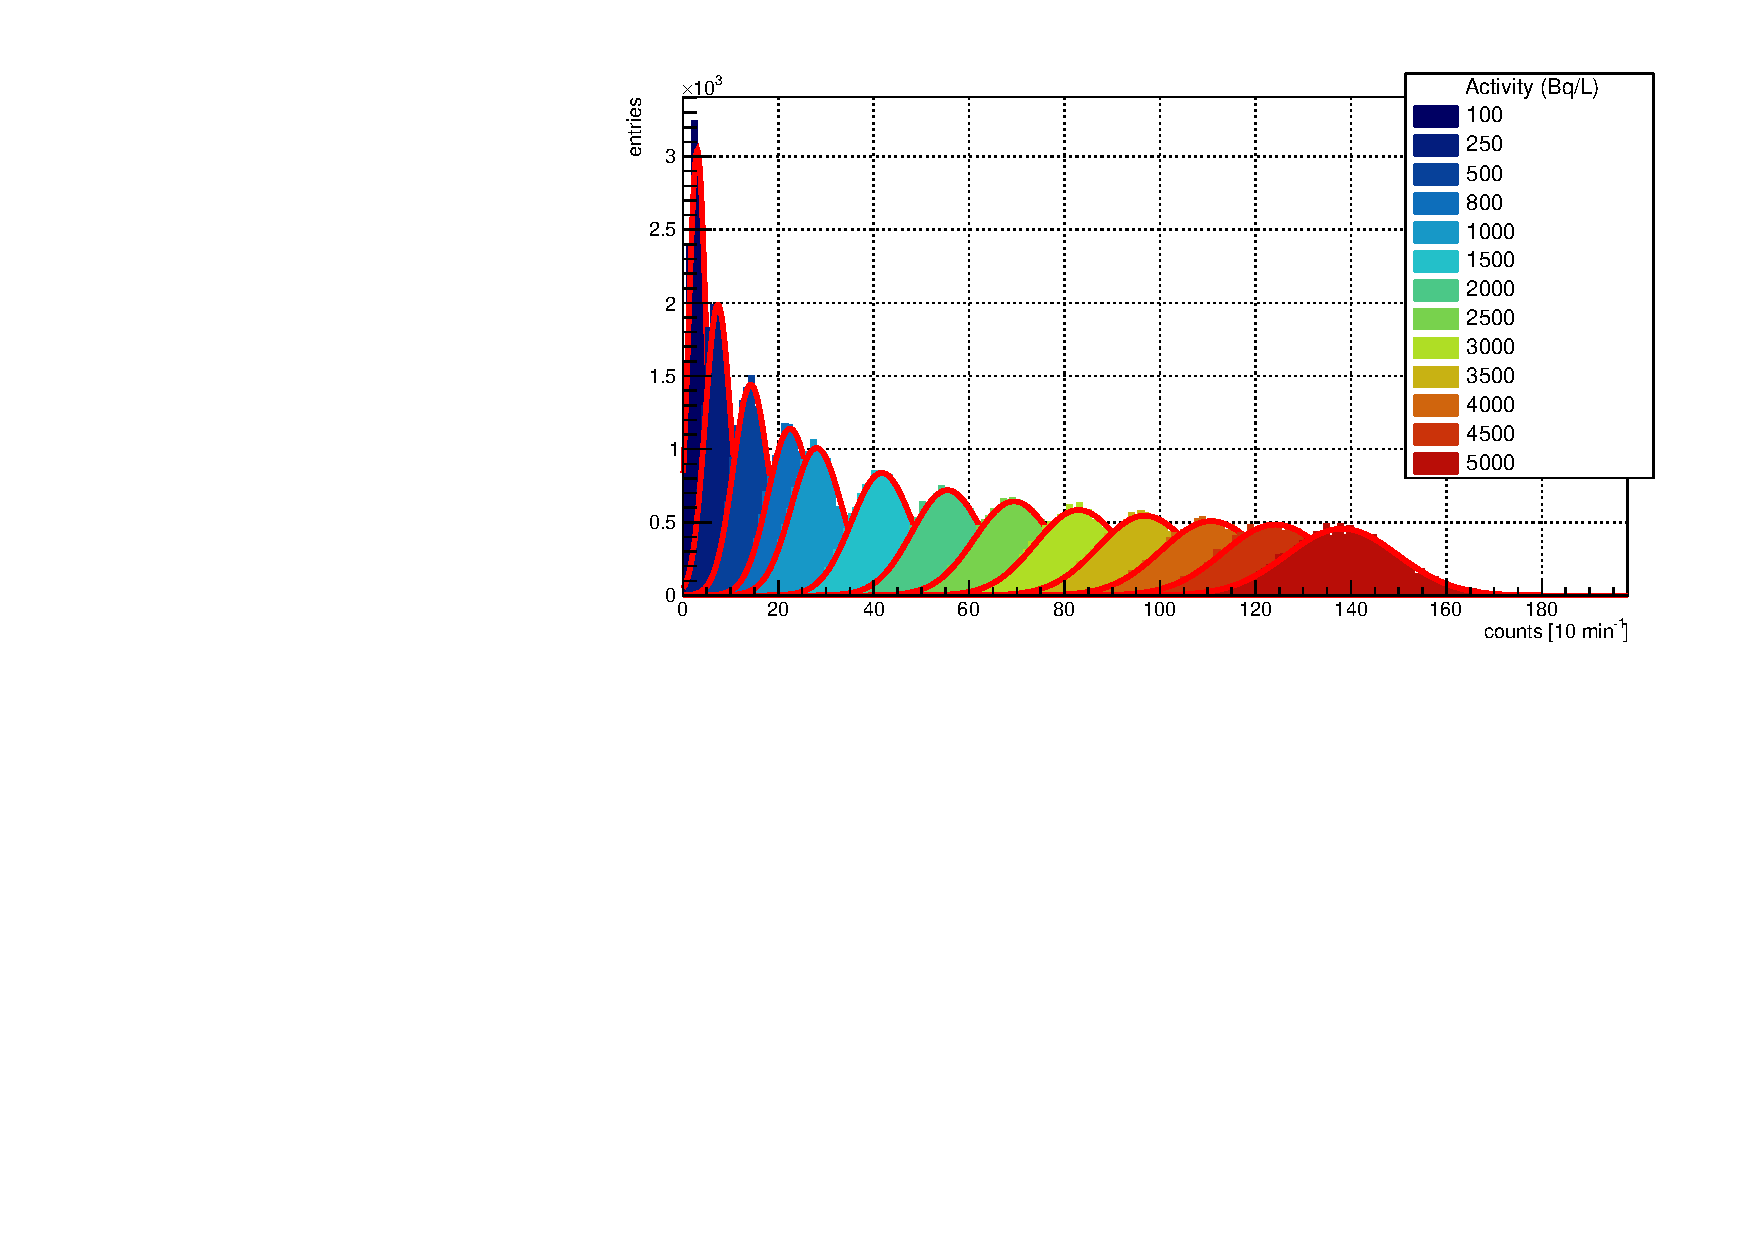
\includegraphics[width=\textwidth]{6Simulations/62TRITIUMMonitor/621TRITIUMIFIC2/Dist_1Det_10min_250BqL_and_Gaus.pdf}  
    \caption{\label{subfig:Dist1Det10Min250BqL}}
    \end{subfigure}
 \caption{a) Simulated of tritium counts measured with a TRITIUM-IFIC-2 prototype, using an integration time of $10~\min$, during three months of measurements ($13248$ measurements for each activity). b) Distribution of these counts for each activities.}
 \label{fig:1Det10Min250BqL}
\end{figure}

\begin{figure}
\centering
    \begin{subfigure}[b]{0.6\textwidth}
    \centering
    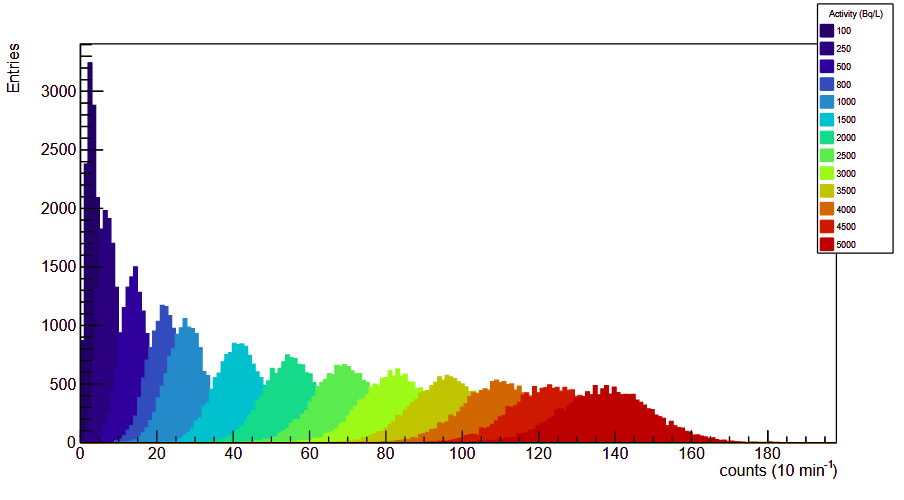
\includegraphics[width=\textwidth]{6Simulations/62TRITIUMMonitor/621TRITIUMIFIC2/Dist_1Det_10min_250BqL.png}  
    \caption{\label{subfig:1Det10min250BqLST}}
    \end{subfigure}
    \hfill
    \begin{subfigure}[b]{0.6\textwidth}
    \centering
    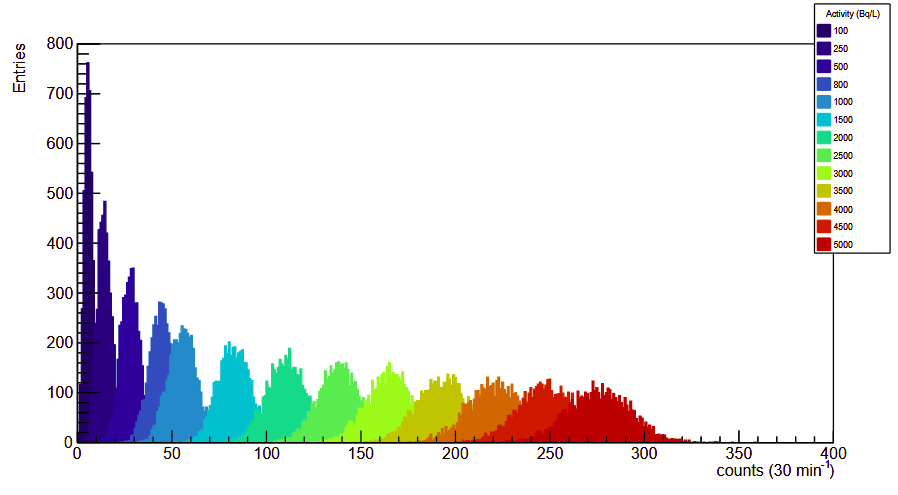
\includegraphics[width=\textwidth]{6Simulations/62TRITIUMMonitor/621TRITIUMIFIC2/Dist_1Det_30min_250BqL.png}  
    \caption{\label{subfig:1Det30min250BqLST}}
    \end{subfigure}
    \hfill
    \begin{subfigure}[b]{0.6\textwidth}
    \centering
    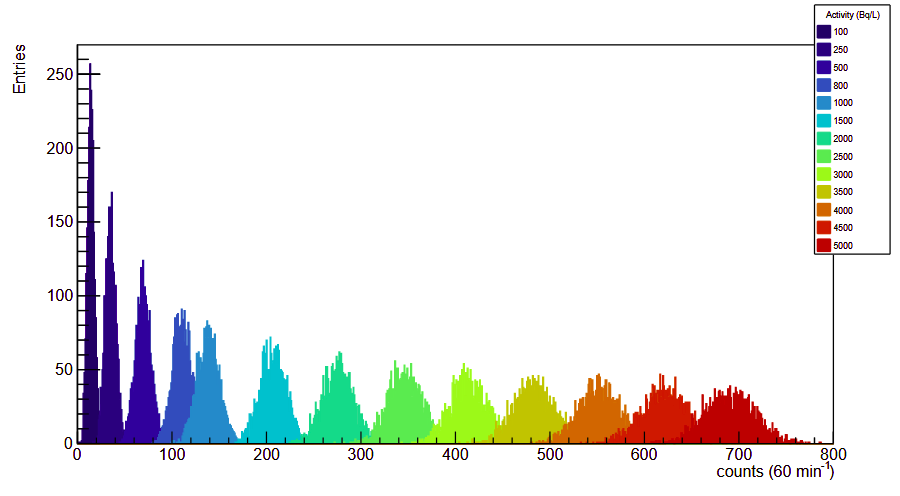
\includegraphics[width=\textwidth]{6Simulations/62TRITIUMMonitor/621TRITIUMIFIC2/Dist_1Det_60min_250BqL.png}  
    \caption{\label{subfig:1Det60min250BqLST}}
    \end{subfigure}
 \caption{Simulation of the distribution of the tritium counts obtained with a TRITIUM-IFIC-2 prototype for different tritium activities during three months of measurements and three different integration times: a)$10~\min$ ($13248$ measurements), b) $30~\min$ ($4416$ measurements) and c) $60~\min$ ($2208$ measurements).}
 \label{fig:1Det250BqLseveralTimes}
\end{figure} 

\begin{figure}
\centering
    \begin{subfigure}[b]{0.6\textwidth}
    \centering
    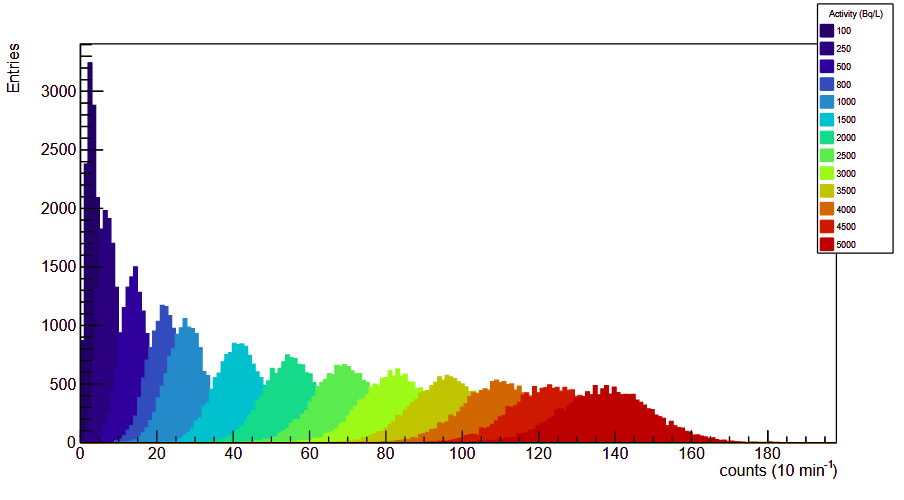
\includegraphics[width=\textwidth]{6Simulations/62TRITIUMMonitor/621TRITIUMIFIC2/Dist_1Det_10min_250BqL.png}  
    \caption{\label{subfig:1Det10min250BqLSD}}
    \end{subfigure}
    \hfill
    \begin{subfigure}[b]{0.6\textwidth}
    \centering
    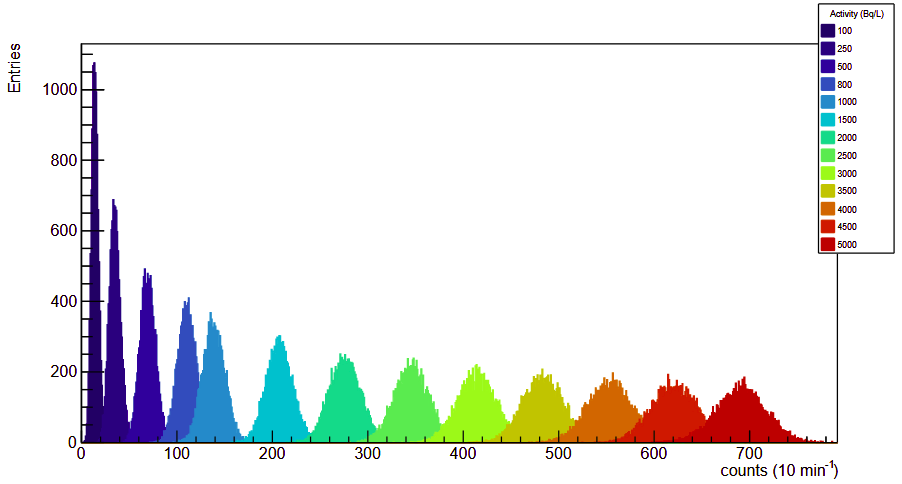
\includegraphics[width=\textwidth]{6Simulations/62TRITIUMMonitor/621TRITIUMIFIC2/Dist_5Det_10min_250BqL.png}  
    \caption{\label{subfig:5Det10min250BqLSD}}
    \end{subfigure}
    \hfill
    \begin{subfigure}[b]{0.6\textwidth}
    \centering
    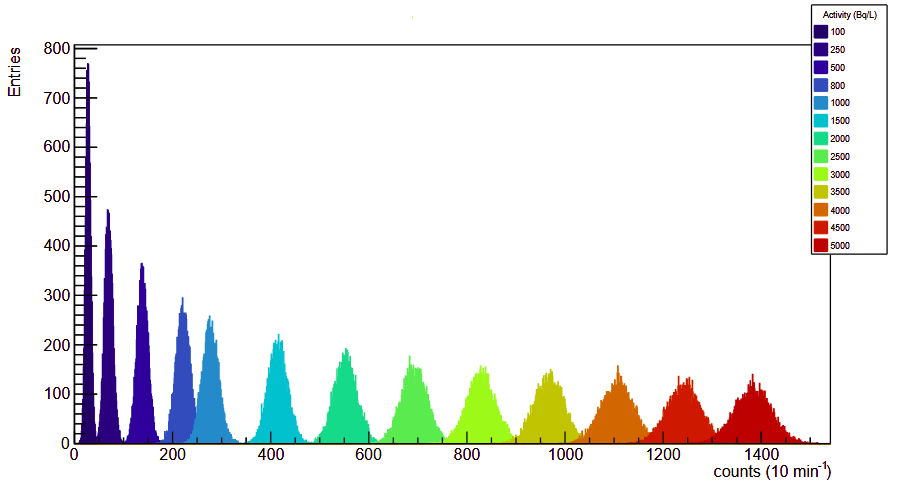
\includegraphics[width=\textwidth]{6Simulations/62TRITIUMMonitor/621TRITIUMIFIC2/Dist_10Det_10min_250BqL.png}  
    \caption{\label{subfig:10Det10min250BqLSD}}
    \end{subfigure}
 \caption{Simulaton of the distribution of the tritium counts during three months using an integration time of $10~\min$ ($13248$ measurements) for different tritium activities and different number of TRITIUM-IFIC-2 modules: a) 1, b) 5 and c) 10.}
 \label{fig:SeveralDet250BqL10min}
\end{figure}

\begin{figure}
\centering
    \begin{subfigure}[b]{0.75\textwidth}
    \centering
    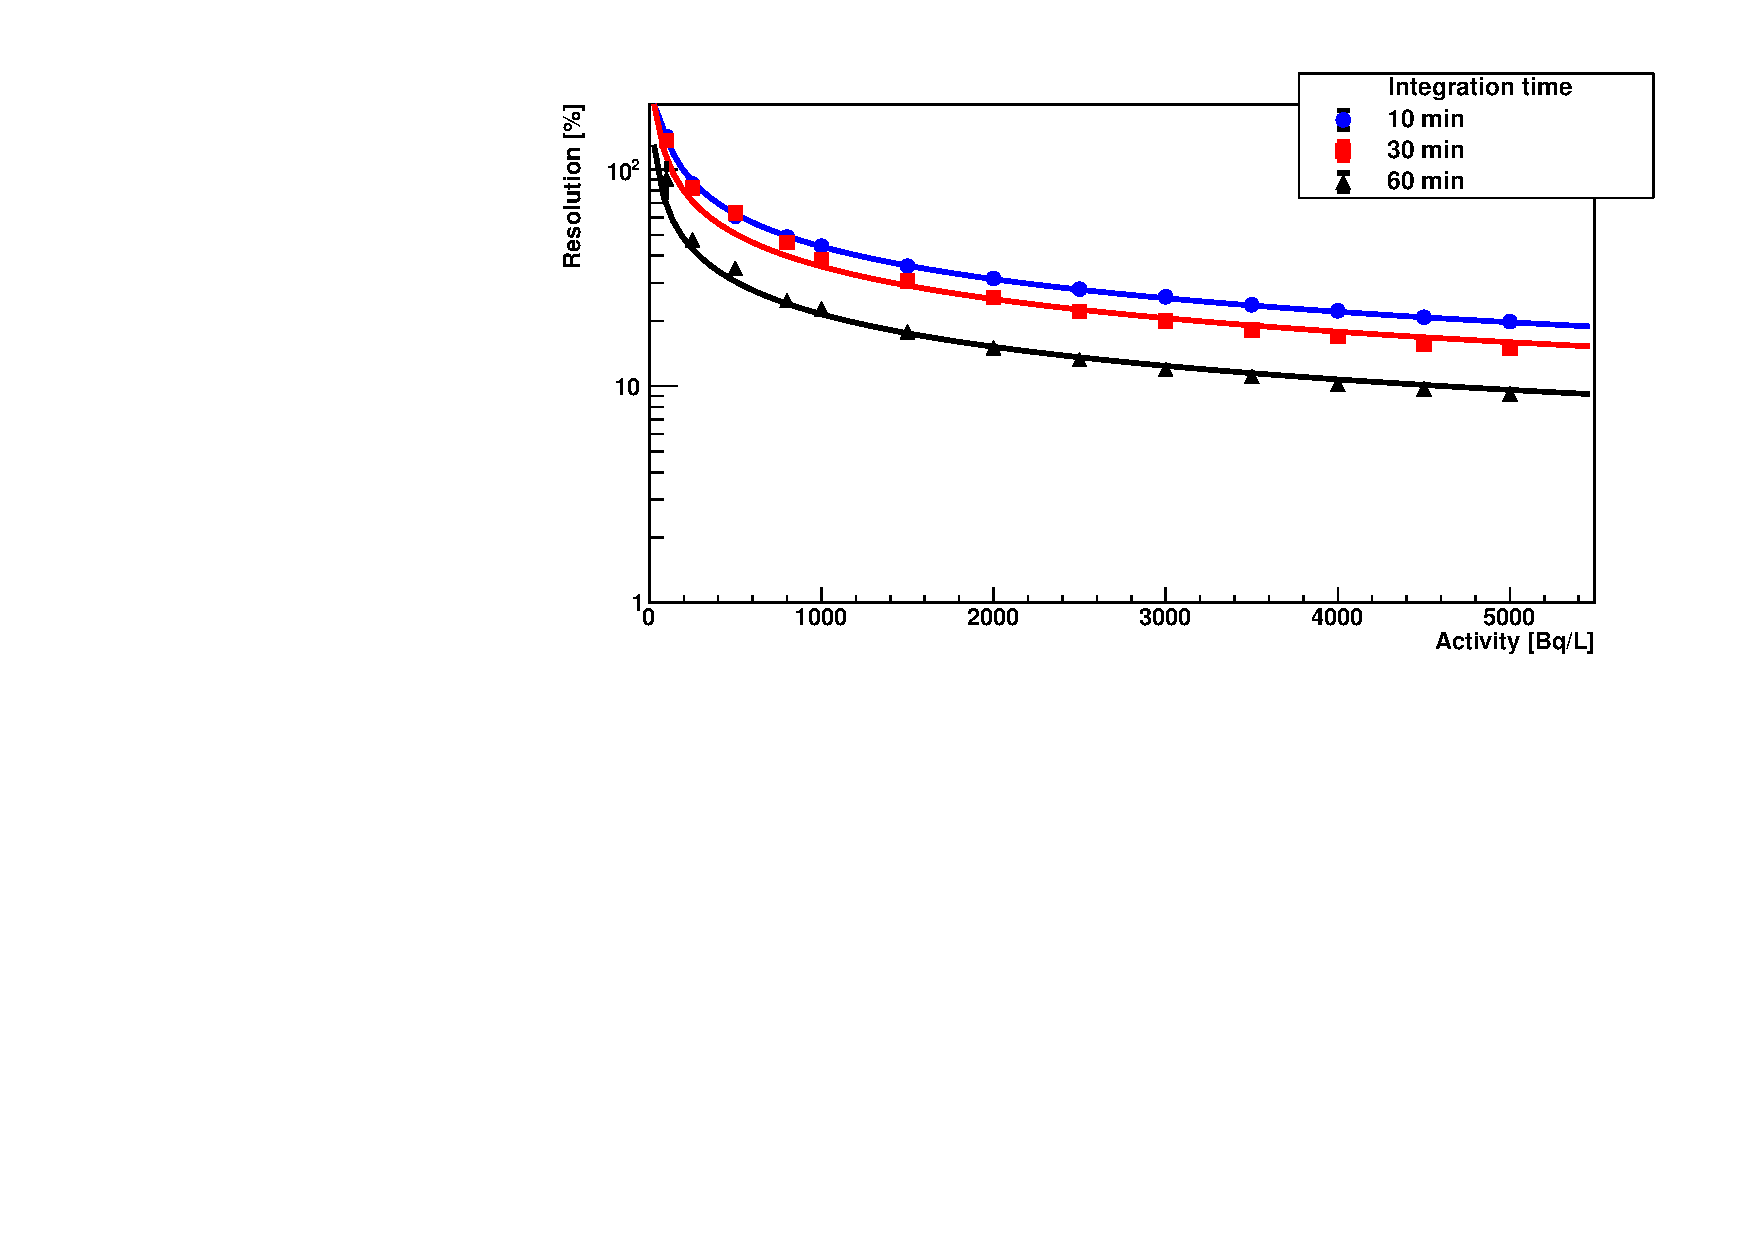
\includegraphics[width=\textwidth]{6Simulations/62TRITIUMMonitor/621TRITIUMIFIC2/Results_Several_Times.pdf}  
    \caption{\label{subfig:ResolutionvsIntegrationCoutingTime}}
    \end{subfigure}
    \hfill
    \begin{subfigure}[b]{0.75\textwidth}
    \centering
    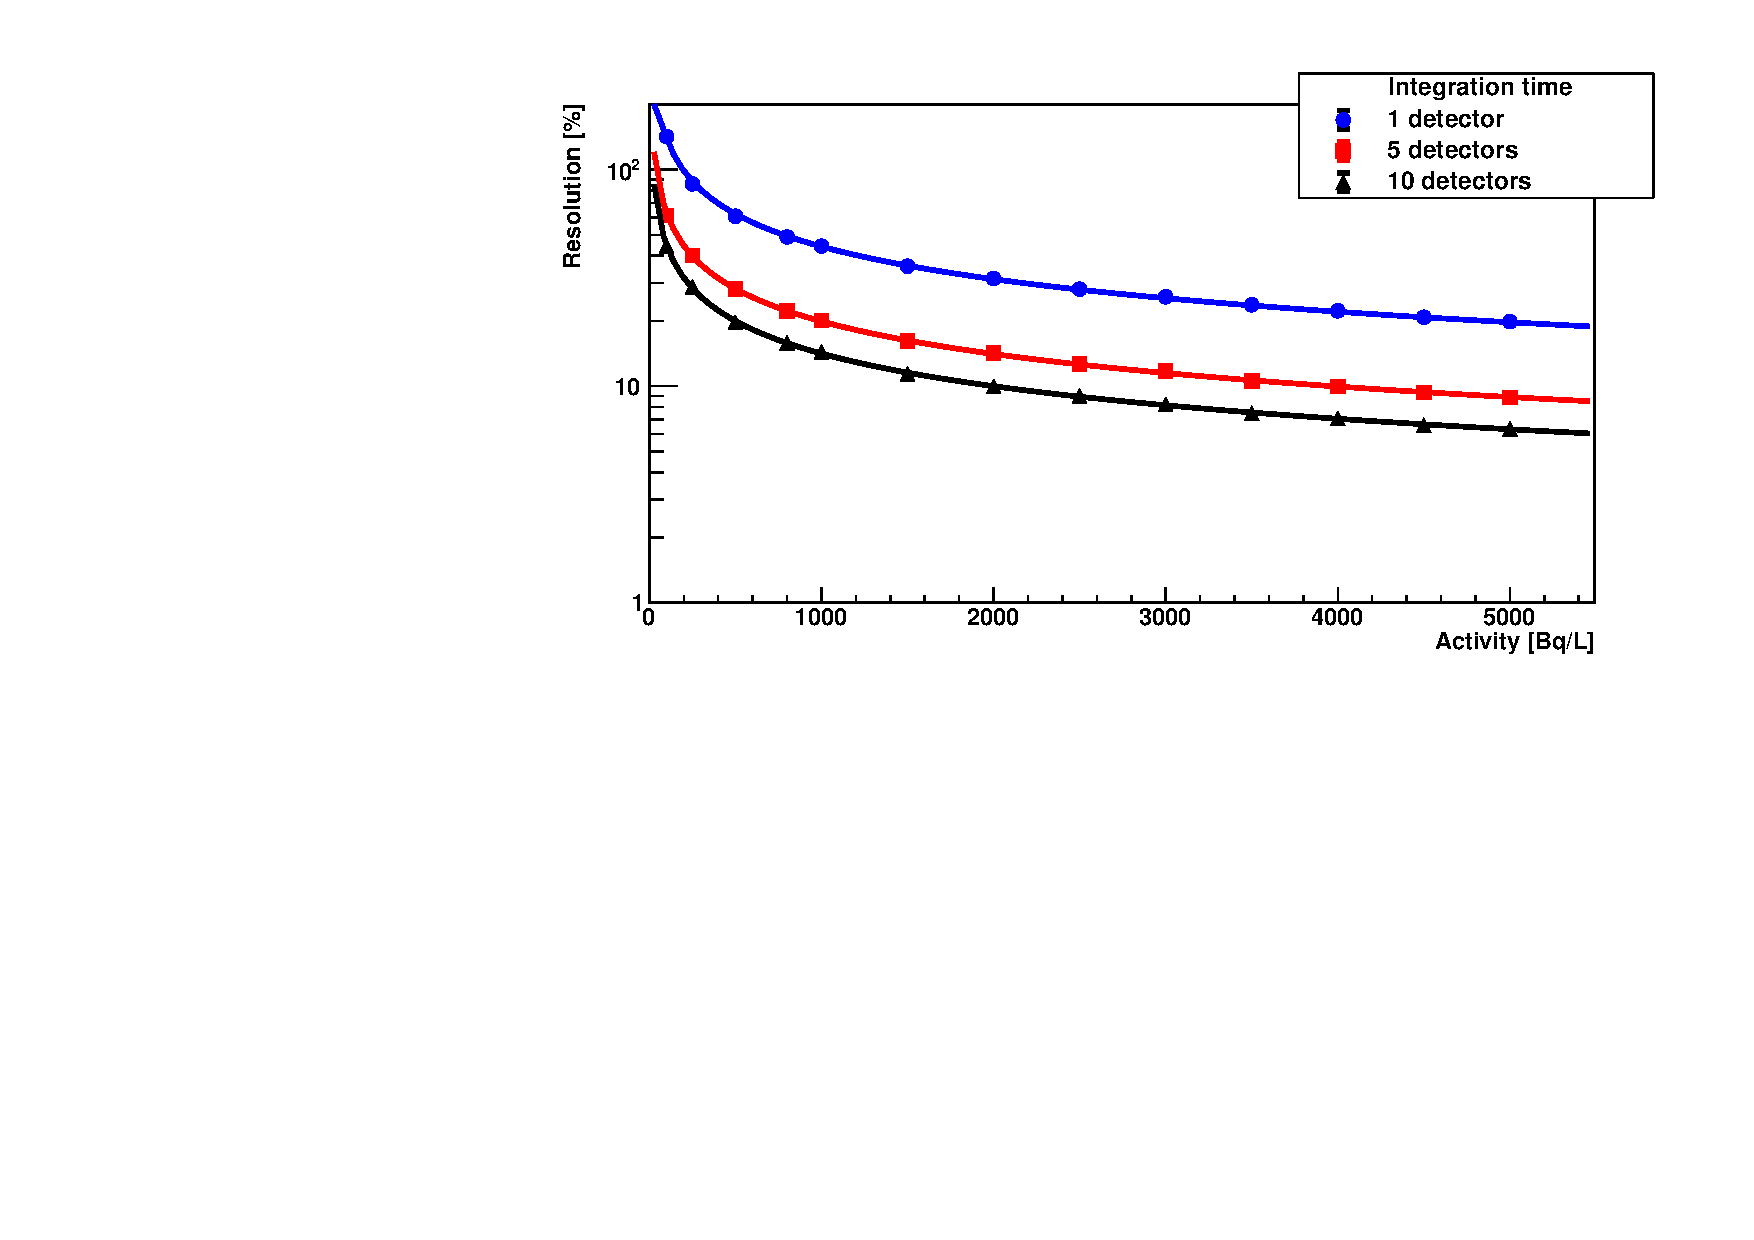
\includegraphics[width=\textwidth]{6Simulations/62TRITIUMMonitor/621TRITIUMIFIC2/Results_Several_Detectors.pdf}  
    \caption{\label{subfig:ResolutionvsNumberDetectors}}
    \end{subfigure}
 \caption{Resolution of the TRITIUM-IFIC-2 prototype as a function of the. a) Integration counting time using 1 TRITIUM-IFIC 2 module. b) Number of modules, using an integration counting time of $10~\min$.}
 \label{fig:Resolution}
\end{figure}

\begin{table}[htbp]
\centering{}%
\begin{tabular}{lccc}
\toprule 
\# of modules & $10~\min$ & $30~\min$ & $60~\min$ \tabularnewline
\midrule
\midrule 
1 & $<1000~\becquerel/\liter$ & $500~\becquerel/\liter$ & $200~\becquerel/\liter$ \tabularnewline
5 & $200~\becquerel/\liter$ & $150~\becquerel/\liter$ & $100~\becquerel/\liter$ \tabularnewline
10 & $150~\becquerel/\liter$ & $100~\becquerel/\liter$ & $\approx 50~\becquerel/\liter$ \tabularnewline
\bottomrule
\end{tabular}
\caption{Difference in activity that can be resolved for the TRITIUM-IFIC-2 prototype, for different integration times and different number of modules.}
\label{tab:DifferentCasesOfTI2}
\end{table}

The decision made by the TRITIUM collaboration is to install 5 TRITIUM-IFIC-2 modules with an integration time of $1~\hour$, with which a MDA of $100~\becquerel/\liter$ is expected to be achieved, as it was seen in Figure \ref{fig:MDATRITIUMmonitor}. With this configurations, differences of $100~\becquerel/\liter$ are expected to be resolved according to the table \ref{tab:DifferentCasesOfTI2}. 

Three TRITIUM-IFIC-2 modules are planned to be installed in Arrocampo dam as soon as possible, which will be used to detect and solve prossible problems when several TRITIUM modules are read out in parallel. In addition, two other TRITIUM-Aveiro prototypes are being built and will be installed soon, to be read out in parallel with the one currently installed.

%Se ha realizado un ajuste lineal del centroide de las gaussianas de los ajustes (y su anchura como error) frente a la actividad usada. El rango utilizado en este caso ha sido mucho mayor debido a

%Tritium detection was studied using only one TRITIUM-IFIC-2 prototype, throguh the simulation of various activities of tritiated water. The integration count time used was $10~\min$ and continuous use of the detector during 3 months was simulated for each activity studied.


%PEORES RESULTADOS SIMULADOS QUE CON AVEIRO PERO MEJORES EXPERIMENTALMENTE. La diferencia debe de estar en que uno usa fibras pulida y limpiadas y el otro no.

%PREPARAR EN BACK UP EN LA PRESENTACIÓN EL CASO PARA 3 DETECTORES, YA QUE SERÁ NUESTRO CASO.














%The simulation of the Tritium-Aveiro prototype is similar to this since the design of both detectors are quite similar. There are two main difference between both simulated prototypes:

%\begin{enumerate}

%\item{} The diameter of the fibers used, which is $1~\mm$ for Tritium-IFIC-2 prototype and $2~\mm$ for Tritium-Aveiro prototype. As the internal volume of the PTFE vessel is filled, this difference imply a difference number of the scintillating fibers used, causing a difference in the signal-background ratio.

%\item{} The photosensors used since, although both are PMTs, the model of the used PMTs is different and it cause a different active area readout, affecting to the tritium detection efficiency. 

%\end{enumerate}